\documentclass[1p]{elsarticle_modified}
%\bibliographystyle{elsarticle-num}

%\usepackage[colorlinks]{hyperref}
%\usepackage{abbrmath_seonhwa} %\Abb, \Ascr, \Acal ,\Abf, \Afrak
\usepackage{amsfonts}
\usepackage{amssymb}
\usepackage{amsmath}
\usepackage{amsthm}
\usepackage{scalefnt}
\usepackage{amsbsy}
\usepackage{kotex}
\usepackage{caption}
\usepackage{subfig}
\usepackage{color}
\usepackage{graphicx}
\usepackage{xcolor} %% white, black, red, green, blue, cyan, magenta, yellow
\usepackage{float}
\usepackage{setspace}
\usepackage{hyperref}

\usepackage{tikz}
\usetikzlibrary{arrows}

\usepackage{multirow}
\usepackage{array} % fixed length table
\usepackage{hhline}

%%%%%%%%%%%%%%%%%%%%%
\makeatletter
\renewcommand*\env@matrix[1][\arraystretch]{%
	\edef\arraystretch{#1}%
	\hskip -\arraycolsep
	\let\@ifnextchar\new@ifnextchar
	\array{*\c@MaxMatrixCols c}}
\makeatother %https://tex.stackexchange.com/questions/14071/how-can-i-increase-the-line-spacing-in-a-matrix
%%%%%%%%%%%%%%%

\usepackage[normalem]{ulem}

\newcommand{\msout}[1]{\ifmmode\text{\sout{\ensuremath{#1}}}\else\sout{#1}\fi}
%SOURCE: \msout is \stkout macro in https://tex.stackexchange.com/questions/20609/strikeout-in-math-mode

\newcommand{\cancel}[1]{
	\ifmmode
	{\color{red}\msout{#1}}
	\else
	{\color{red}\sout{#1}}
	\fi
}

\newcommand{\add}[1]{
	{\color{blue}\uwave{#1}}
}

\newcommand{\replace}[2]{
	\ifmmode
	{\color{red}\msout{#1}}{\color{blue}\uwave{#2}}
	\else
	{\color{red}\sout{#1}}{\color{blue}\uwave{#2}}
	\fi
}

\newcommand{\Sol}{\mathcal{S}} %segment
\newcommand{\D}{D} %diagram
\newcommand{\A}{\mathcal{A}} %arc


%%%%%%%%%%%%%%%%%%%%%%%%%%%%%5 test

\def\sl{\operatorname{\textup{SL}}(2,\Cbb)}
\def\psl{\operatorname{\textup{PSL}}(2,\Cbb)}
\def\quan{\mkern 1mu \triangleright \mkern 1mu}

\theoremstyle{definition}
\newtheorem{thm}{Theorem}[section]
\newtheorem{prop}[thm]{Proposition}
\newtheorem{lem}[thm]{Lemma}
\newtheorem{ques}[thm]{Question}
\newtheorem{cor}[thm]{Corollary}
\newtheorem{defn}[thm]{Definition}
\newtheorem{exam}[thm]{Example}
\newtheorem{rmk}[thm]{Remark}
\newtheorem{alg}[thm]{Algorithm}

\newcommand{\I}{\sqrt{-1}}
\begin{document}

%\begin{frontmatter}
%
%\title{Boundary parabolic representations of knots up to 8 crossings}
%
%%% Group authors per affiliation:
%\author{Yunhi Cho} 
%\address{Department of Mathematics, University of Seoul, Seoul, Korea}
%\ead{yhcho@uos.ac.kr}
%
%
%\author{Seonhwa Kim} %\fnref{s_kim}}
%\address{Center for Geometry and Physics, Institute for Basic Science, Pohang, 37673, Korea}
%\ead{ryeona17@ibs.re.kr}
%
%\author{Hyuk Kim}
%\address{Department of Mathematical Sciences, Seoul National University, Seoul 08826, Korea}
%\ead{hyukkim@snu.ac.kr}
%
%\author{Seokbeom Yoon}
%\address{Department of Mathematical Sciences, Seoul National University, Seoul, 08826,  Korea}
%\ead{sbyoon15@snu.ac.kr}
%
%\begin{abstract}
%We find all boundary parabolic representation of knots up to 8 crossings.
%
%\end{abstract}
%\begin{keyword}
%    \MSC[2010] 57M25 
%\end{keyword}
%
%\end{frontmatter}

%\linenumbers
%\tableofcontents
%
\newcommand\colored[1]{\textcolor{white}{\rule[-0.35ex]{0.8em}{1.4ex}}\kern-0.8em\color{red} #1}%
%\newcommand\colored[1]{\textcolor{white}{ #1}\kern-2.17ex	\textcolor{white}{ #1}\kern-1.81ex	\textcolor{white}{ #1}\kern-2.15ex\color{red}#1	}

{\Large $\underline{11a_{221}~(K11a_{221})}$}

\setlength{\tabcolsep}{10pt}
\renewcommand{\arraystretch}{1.6}
\vspace{1cm}\begin{tabular}{m{100pt}>{\centering\arraybackslash}m{274pt}}
\multirow{5}{120pt}{
	\centering
	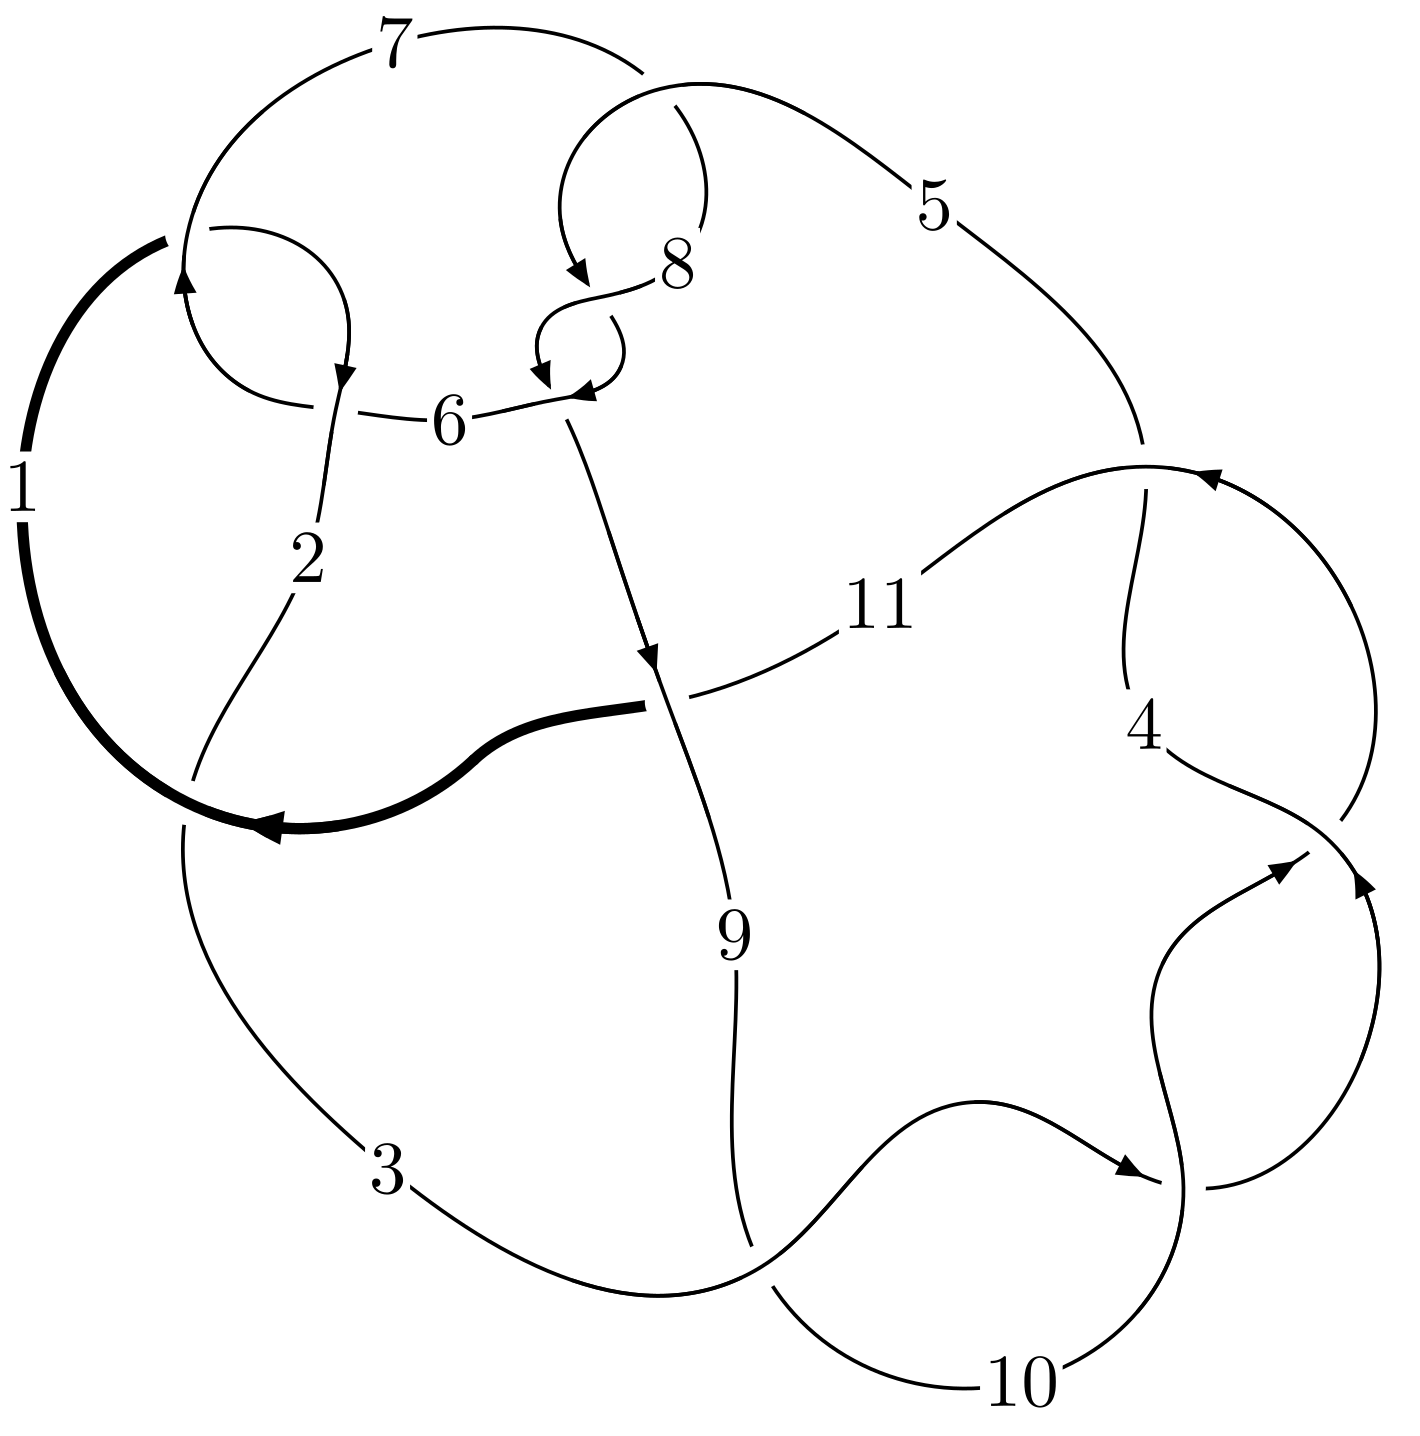
\includegraphics[width=112pt]{../../../GIT/diagram.site/Diagrams/png/470_11a_221.png}\\
\ \ \ A knot diagram\footnotemark}&
\allowdisplaybreaks
\textbf{Linearized knot diagam} \\
\cline{2-2}
 &
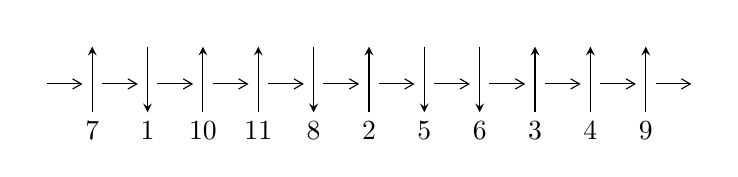
\begin{tikzpicture}[x=20pt, y=17pt]
	% nodes
	\node (C0) at (0, 0) {};
	\node (C1) at (1, 0) {};
	\node (C1U) at (1, +1) {};
	\node (C1D) at (1, -1) {7};

	\node (C2) at (2, 0) {};
	\node (C2U) at (2, +1) {};
	\node (C2D) at (2, -1) {1};

	\node (C3) at (3, 0) {};
	\node (C3U) at (3, +1) {};
	\node (C3D) at (3, -1) {10};

	\node (C4) at (4, 0) {};
	\node (C4U) at (4, +1) {};
	\node (C4D) at (4, -1) {11};

	\node (C5) at (5, 0) {};
	\node (C5U) at (5, +1) {};
	\node (C5D) at (5, -1) {8};

	\node (C6) at (6, 0) {};
	\node (C6U) at (6, +1) {};
	\node (C6D) at (6, -1) {2};

	\node (C7) at (7, 0) {};
	\node (C7U) at (7, +1) {};
	\node (C7D) at (7, -1) {5};

	\node (C8) at (8, 0) {};
	\node (C8U) at (8, +1) {};
	\node (C8D) at (8, -1) {6};

	\node (C9) at (9, 0) {};
	\node (C9U) at (9, +1) {};
	\node (C9D) at (9, -1) {3};

	\node (C10) at (10, 0) {};
	\node (C10U) at (10, +1) {};
	\node (C10D) at (10, -1) {4};

	\node (C11) at (11, 0) {};
	\node (C11U) at (11, +1) {};
	\node (C11D) at (11, -1) {9};
	\node (C12) at (12, 0) {};

	% arrows
	\draw[->,>={angle 60}]
	(C0) edge (C1) (C1) edge (C2) (C2) edge (C3) (C3) edge (C4) (C4) edge (C5) (C5) edge (C6) (C6) edge (C7) (C7) edge (C8) (C8) edge (C9) (C9) edge (C10) (C10) edge (C11) (C11) edge (C12) ;	\draw[->,>=stealth]
	(C1D) edge (C1U) (C2U) edge (C2D) (C3D) edge (C3U) (C4D) edge (C4U) (C5U) edge (C5D) (C6D) edge (C6U) (C7U) edge (C7D) (C8U) edge (C8D) (C9D) edge (C9U) (C10D) edge (C10U) (C11D) edge (C11U) ;
	\end{tikzpicture} \\
\hhline{~~} \\& 
\textbf{Solving Sequence} \\ \cline{2-2} 
 &
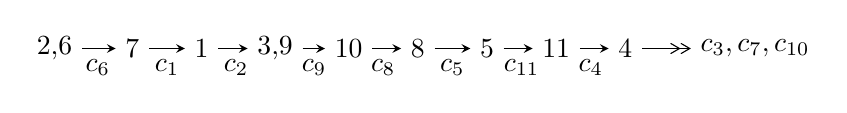
\begin{tikzpicture}[x=25pt, y=7pt]
	% node
	\node (A0) at (-1/8, 0) {2,6};
	\node (A1) at (1, 0) {7};
	\node (A2) at (2, 0) {1};
	\node (A3) at (49/16, 0) {3,9};
	\node (A4) at (33/8, 0) {10};
	\node (A5) at (41/8, 0) {8};
	\node (A6) at (49/8, 0) {5};
	\node (A7) at (57/8, 0) {11};
	\node (A8) at (65/8, 0) {4};
	\node (C1) at (1/2, -1) {$c_{6}$};
	\node (C2) at (3/2, -1) {$c_{1}$};
	\node (C3) at (5/2, -1) {$c_{2}$};
	\node (C4) at (29/8, -1) {$c_{9}$};
	\node (C5) at (37/8, -1) {$c_{8}$};
	\node (C6) at (45/8, -1) {$c_{5}$};
	\node (C7) at (53/8, -1) {$c_{11}$};
	\node (C8) at (61/8, -1) {$c_{4}$};
	\node (A9) at (10, 0) {$c_{3},c_{7},c_{10}$};

	% edge
	\draw[->,>=stealth]	
	(A0) edge (A1) (A1) edge (A2) (A2) edge (A3) (A3) edge (A4) (A4) edge (A5) (A5) edge (A6) (A6) edge (A7) (A7) edge (A8) ;
	\draw[->>,>={angle 60}]	
	(A8) edge (A9);
\end{tikzpicture} \\ 

\end{tabular} \\

\footnotetext{
The image of knot diagram is generated by the software ``\textbf{Draw programme}" developed by Andrew Bartholomew(\url{http://www.layer8.co.uk/maths/draw/index.htm\#Running-draw}), where we modified some parts for our purpose(\url{https://github.com/CATsTAILs/LinksPainter}).
}\phantom \\ \newline 
\centering \textbf{Ideals for irreducible components\footnotemark of $X_{\text{par}}$} 
 
\begin{align*}
I^u_{1}&=\langle 
2.58574\times10^{22} u^{40}+1.94775\times10^{22} u^{39}+\cdots+4.92580\times10^{22} b+1.64635\times10^{22},\\
\phantom{I^u_{1}}&\phantom{= \langle  }-8.09547\times10^{21} u^{40}+5.99125\times10^{21} u^{39}+\cdots+1.97032\times10^{23} a+1.41113\times10^{23},\;u^{41}+u^{40}+\cdots- u^2+4\rangle \\
\\
I^v_{1}&=\langle 
a,\;b-1,\;v^2+v-1\rangle \\
\end{align*}
\raggedright * 2 irreducible components of $\dim_{\mathbb{C}}=0$, with total 43 representations.\\
\footnotetext{All coefficients of polynomials are rational numbers. But the coefficients are sometimes approximated in decimal forms when there is not enough margin.}
\newpage
\renewcommand{\arraystretch}{1}
\centering \section*{I. $I^u_{1}= \langle 2.59\times10^{22} u^{40}+1.95\times10^{22} u^{39}+\cdots+4.93\times10^{22} b+1.65\times10^{22},\;-8.10\times10^{21} u^{40}+5.99\times10^{21} u^{39}+\cdots+1.97\times10^{23} a+1.41\times10^{23},\;u^{41}+u^{40}+\cdots- u^2+4 \rangle$}
\flushleft \textbf{(i) Arc colorings}\\
\begin{tabular}{m{7pt} m{180pt} m{7pt} m{180pt} }
\flushright $a_{2}=$&$\begin{pmatrix}0\\u\end{pmatrix}$ \\
\flushright $a_{6}=$&$\begin{pmatrix}1\\0\end{pmatrix}$ \\
\flushright $a_{7}=$&$\begin{pmatrix}1\\- u^2\end{pmatrix}$ \\
\flushright $a_{1}=$&$\begin{pmatrix}- u\\u^3+u\end{pmatrix}$ \\
\flushright $a_{3}=$&$\begin{pmatrix}- u^3\\u^5+u^3+u\end{pmatrix}$ \\
\flushright $a_{9}=$&$\begin{pmatrix}0.0410870 u^{40}-0.0304075 u^{39}+\cdots+2.81027 u-0.716193\\-0.524938 u^{40}-0.395417 u^{39}+\cdots-2.01455 u-0.334229\end{pmatrix}$ \\
\flushright $a_{10}=$&$\begin{pmatrix}-0.467248 u^{40}-0.157588 u^{39}+\cdots+1.16973 u-0.888909\\-0.369945 u^{40}-0.267670 u^{39}+\cdots-1.30888 u-0.201698\end{pmatrix}$ \\
\flushright $a_{8}=$&$\begin{pmatrix}-0.483851 u^{40}-0.425824 u^{39}+\cdots+0.795719 u-1.05042\\-0.524938 u^{40}-0.395417 u^{39}+\cdots-2.01455 u-0.334229\end{pmatrix}$ \\
\flushright $a_{5}=$&$\begin{pmatrix}-0.483851 u^{40}-0.425824 u^{39}+\cdots+0.795719 u-1.05042\\0.0665166 u^{40}+0.364543 u^{39}+\cdots+0.0791500 u+0.566335\end{pmatrix}$ \\
\flushright $a_{11}=$&$\begin{pmatrix}-0.526272 u^{40}-0.615949 u^{39}+\cdots-0.847432 u-2.92163\\-0.400524 u^{40}+0.0414901 u^{39}+\cdots-0.0904238 u-0.792124\end{pmatrix}$ \\
\flushright $a_{4}=$&$\begin{pmatrix}0.405800 u^{40}+0.723766 u^{39}+\cdots-0.573295 u+3.61744\\0.260796 u^{40}+0.239160 u^{39}+\cdots+0.874019 u+0.565373\end{pmatrix}$\\ \flushright $a_{4}=$&$\begin{pmatrix}0.405800 u^{40}+0.723766 u^{39}+\cdots-0.573295 u+3.61744\\0.260796 u^{40}+0.239160 u^{39}+\cdots+0.874019 u+0.565373\end{pmatrix}$\\&\end{tabular}
\flushleft \textbf{(ii) Obstruction class $= -1$}\\~\\
\flushleft \textbf{(iii) Cusp Shapes $= -\frac{3657064353645414395094}{24629024686271213113517} u^{40}-\frac{45534143106179376249815}{24629024686271213113517} u^{39}+\cdots+\frac{159536480684658033188744}{24629024686271213113517} u-\frac{110862013990068277848729}{24629024686271213113517}$}\\~\\
\newpage\renewcommand{\arraystretch}{1}
\flushleft \textbf{(iv) u-Polynomials at the component}\newline \\
\begin{tabular}{m{50pt}|m{274pt}}
Crossings & \hspace{64pt}u-Polynomials at each crossing \\
\hline $$\begin{aligned}c_{1},c_{6}\end{aligned}$$&$\begin{aligned}
&u^{41}+u^{40}+\cdots- u^2+4
\end{aligned}$\\
\hline $$\begin{aligned}c_{2}\end{aligned}$$&$\begin{aligned}
&u^{41}+15 u^{40}+\cdots+8 u-16
\end{aligned}$\\
\hline $$\begin{aligned}c_{3},c_{4},c_{9}\\c_{10}\end{aligned}$$&$\begin{aligned}
&u^{41}-2 u^{40}+\cdots- u-1
\end{aligned}$\\
\hline $$\begin{aligned}c_{5},c_{7},c_{8}\end{aligned}$$&$\begin{aligned}
&u^{41}-3 u^{40}+\cdots-6 u+1
\end{aligned}$\\
\hline $$\begin{aligned}c_{11}\end{aligned}$$&$\begin{aligned}
&u^{41}+12 u^{40}+\cdots-503 u-73
\end{aligned}$\\
\hline
\end{tabular}\\~\\
\newpage\renewcommand{\arraystretch}{1}
\flushleft \textbf{(v) Riley Polynomials at the component}\newline \\
\begin{tabular}{m{50pt}|m{274pt}}
Crossings & \hspace{64pt}Riley Polynomials at each crossing \\
\hline $$\begin{aligned}c_{1},c_{6}\end{aligned}$$&$\begin{aligned}
&y^{41}+15 y^{40}+\cdots+8 y-16
\end{aligned}$\\
\hline $$\begin{aligned}c_{2}\end{aligned}$$&$\begin{aligned}
&y^{41}+19 y^{40}+\cdots+16416 y-256
\end{aligned}$\\
\hline $$\begin{aligned}c_{3},c_{4},c_{9}\\c_{10}\end{aligned}$$&$\begin{aligned}
&y^{41}-48 y^{40}+\cdots+3 y-1
\end{aligned}$\\
\hline $$\begin{aligned}c_{5},c_{7},c_{8}\end{aligned}$$&$\begin{aligned}
&y^{41}-35 y^{40}+\cdots+62 y-1
\end{aligned}$\\
\hline $$\begin{aligned}c_{11}\end{aligned}$$&$\begin{aligned}
&y^{41}-12 y^{40}+\cdots+23351 y-5329
\end{aligned}$\\
\hline
\end{tabular}\\~\\
\newpage\flushleft \textbf{(vi) Complex Volumes and Cusp Shapes}
$$\begin{array}{c|c|c}  
\text{Solutions to }I^u_{1}& \I (\text{vol} + \sqrt{-1}CS) & \text{Cusp shape}\\
 \hline 
\begin{aligned}
u &= -0.122270 + 1.001390 I \\
a &= -0.003929 - 0.811821 I \\
b &= \phantom{-}0.562217 + 0.598084 I\end{aligned}
 & \phantom{-}4.86048 - 2.17709 I & \phantom{-}3.44971 + 3.79306 I \\ \hline\begin{aligned}
u &= -0.122270 - 1.001390 I \\
a &= -0.003929 + 0.811821 I \\
b &= \phantom{-}0.562217 - 0.598084 I\end{aligned}
 & \phantom{-}4.86048 + 2.17709 I & \phantom{-}3.44971 - 3.79306 I \\ \hline\begin{aligned}
u &= \phantom{-}0.551581 + 0.859891 I \\
a &= \phantom{-}0.449439 + 1.057630 I \\
b &= \phantom{-}0.181877 - 0.689383 I\end{aligned}
 & \phantom{-}0.32453 + 2.20665 I & \phantom{-}2.42130 - 3.15065 I \\ \hline\begin{aligned}
u &= \phantom{-}0.551581 - 0.859891 I \\
a &= \phantom{-}0.449439 - 1.057630 I \\
b &= \phantom{-}0.181877 + 0.689383 I\end{aligned}
 & \phantom{-}0.32453 - 2.20665 I & \phantom{-}2.42130 + 3.15065 I \\ \hline\begin{aligned}
u &= \phantom{-}1.02478\phantom{ +0.000000I} \\
a &= -0.908342\phantom{ +0.000000I} \\
b &= \phantom{-}1.33636\phantom{ +0.000000I}\end{aligned}
 & \phantom{-}2.95183\phantom{ +0.000000I} & \phantom{-}3.34750\phantom{ +0.000000I} \\ \hline\begin{aligned}
u &= -0.679117 + 0.681890 I \\
a &= \phantom{-}0.700414 - 1.106750 I \\
b &= \phantom{-}0.001662 + 0.650682 I\end{aligned}
 & \phantom{-}2.92066 + 0.49867 I & \phantom{-}9.33255 - 1.40381 I \\ \hline\begin{aligned}
u &= -0.679117 - 0.681890 I \\
a &= \phantom{-}0.700414 + 1.106750 I \\
b &= \phantom{-}0.001662 - 0.650682 I\end{aligned}
 & \phantom{-}2.92066 - 0.49867 I & \phantom{-}9.33255 + 1.40381 I \\ \hline\begin{aligned}
u &= -0.545090 + 0.785733 I \\
a &= -0.69091 + 2.59079 I \\
b &= -1.209880 - 0.257619 I\end{aligned}
 & \phantom{-}7.70281 - 1.46253 I & \phantom{-}4.97551 + 4.38414 I \\ \hline\begin{aligned}
u &= -0.545090 - 0.785733 I \\
a &= -0.69091 - 2.59079 I \\
b &= -1.209880 + 0.257619 I\end{aligned}
 & \phantom{-}7.70281 + 1.46253 I & \phantom{-}4.97551 - 4.38414 I \\ \hline\begin{aligned}
u &= \phantom{-}0.815378 + 0.666881 I \\
a &= \phantom{-}0.75804 + 1.25639 I \\
b &= -0.085807 - 0.724003 I\end{aligned}
 & \phantom{-}11.08220 - 2.09439 I & \phantom{-}10.58118 + 0.49911 I\\
 \hline 
 \end{array}$$\newpage$$\begin{array}{c|c|c}  
\text{Solutions to }I^u_{1}& \I (\text{vol} + \sqrt{-1}CS) & \text{Cusp shape}\\
 \hline 
\begin{aligned}
u &= \phantom{-}0.815378 - 0.666881 I \\
a &= \phantom{-}0.75804 - 1.25639 I \\
b &= -0.085807 + 0.724003 I\end{aligned}
 & \phantom{-}11.08220 + 2.09439 I & \phantom{-}10.58118 - 0.49911 I \\ \hline\begin{aligned}
u &= \phantom{-}0.925345 + 0.534295 I \\
a &= -0.848621 - 0.304695 I \\
b &= \phantom{-}1.281480 + 0.256105 I\end{aligned}
 & -1.06929 - 3.78517 I & \phantom{-}3.33312 + 5.32313 I \\ \hline\begin{aligned}
u &= \phantom{-}0.925345 - 0.534295 I \\
a &= -0.848621 + 0.304695 I \\
b &= \phantom{-}1.281480 - 0.256105 I\end{aligned}
 & -1.06929 + 3.78517 I & \phantom{-}3.33312 - 5.32313 I \\ \hline\begin{aligned}
u &= \phantom{-}0.512185 + 0.958100 I \\
a &= -0.69987 - 1.88985 I \\
b &= -1.298390 + 0.245537 I\end{aligned}
 & -1.14433 + 2.71303 I & \phantom{-}3.06796 - 2.16565 I \\ \hline\begin{aligned}
u &= \phantom{-}0.512185 - 0.958100 I \\
a &= -0.69987 + 1.88985 I \\
b &= -1.298390 - 0.245537 I\end{aligned}
 & -1.14433 - 2.71303 I & \phantom{-}3.06796 + 2.16565 I \\ \hline\begin{aligned}
u &= \phantom{-}0.471678 + 0.778273 I \\
a &= -0.539722 - 0.459733 I \\
b &= \phantom{-}1.018830 + 0.371555 I\end{aligned}
 & -0.495471 + 1.323540 I & \phantom{-}2.90171 - 5.22285 I \\ \hline\begin{aligned}
u &= \phantom{-}0.471678 - 0.778273 I \\
a &= -0.539722 + 0.459733 I \\
b &= \phantom{-}1.018830 - 0.371555 I\end{aligned}
 & -0.495471 - 1.323540 I & \phantom{-}2.90171 + 5.22285 I \\ \hline\begin{aligned}
u &= -0.579330 + 0.928710 I \\
a &= -0.625557 + 0.571406 I \\
b &= \phantom{-}1.082590 - 0.468575 I\end{aligned}
 & \phantom{-}7.20747 - 3.04463 I & \phantom{-}5.27357 + 2.39823 I \\ \hline\begin{aligned}
u &= -0.579330 - 0.928710 I \\
a &= -0.625557 - 0.571406 I \\
b &= \phantom{-}1.082590 + 0.468575 I\end{aligned}
 & \phantom{-}7.20747 + 3.04463 I & \phantom{-}5.27357 - 2.39823 I \\ \hline\begin{aligned}
u &= -0.790308 + 0.341056 I \\
a &= -0.772495 + 0.188053 I \\
b &= \phantom{-}1.220600 - 0.156477 I\end{aligned}
 & -2.45808 + 0.68070 I & -0.75996 + 1.22832 I\\
 \hline 
 \end{array}$$\newpage$$\begin{array}{c|c|c}  
\text{Solutions to }I^u_{1}& \I (\text{vol} + \sqrt{-1}CS) & \text{Cusp shape}\\
 \hline 
\begin{aligned}
u &= -0.790308 - 0.341056 I \\
a &= -0.772495 - 0.188053 I \\
b &= \phantom{-}1.220600 + 0.156477 I\end{aligned}
 & -2.45808 - 0.68070 I & -0.75996 - 1.22832 I \\ \hline\begin{aligned}
u &= -0.637944 + 0.967189 I \\
a &= \phantom{-}0.396872 - 1.193270 I \\
b &= \phantom{-}0.182840 + 0.800800 I\end{aligned}
 & \phantom{-}2.06145 - 5.60392 I & \phantom{-}6.28993 + 7.67426 I \\ \hline\begin{aligned}
u &= -0.637944 - 0.967189 I \\
a &= \phantom{-}0.396872 + 1.193270 I \\
b &= \phantom{-}0.182840 - 0.800800 I\end{aligned}
 & \phantom{-}2.06145 + 5.60392 I & \phantom{-}6.28993 - 7.67426 I \\ \hline\begin{aligned}
u &= -1.003890 + 0.629446 I \\
a &= -0.896695 + 0.361308 I \\
b &= \phantom{-}1.320330 - 0.305527 I\end{aligned}
 & \phantom{-}6.66704 + 5.82869 I & \phantom{-}5.58070 - 3.39540 I \\ \hline\begin{aligned}
u &= -1.003890 - 0.629446 I \\
a &= -0.896695 - 0.361308 I \\
b &= \phantom{-}1.320330 + 0.305527 I\end{aligned}
 & \phantom{-}6.66704 - 5.82869 I & \phantom{-}5.58070 + 3.39540 I \\ \hline\begin{aligned}
u &= -0.070929 + 1.209930 I \\
a &= -0.919362 + 0.220397 I \\
b &= -1.42404 - 0.03377 I\end{aligned}
 & -7.93550 - 1.94462 I & -3.70499 + 3.68184 I \\ \hline\begin{aligned}
u &= -0.070929 - 1.209930 I \\
a &= -0.919362 - 0.220397 I \\
b &= -1.42404 + 0.03377 I\end{aligned}
 & -7.93550 + 1.94462 I & -3.70499 - 3.68184 I \\ \hline\begin{aligned}
u &= -0.028788 + 0.761611 I \\
a &= -0.057057 + 0.439082 I \\
b &= \phantom{-}0.642973 - 0.323659 I\end{aligned}
 & -1.37623 + 1.10536 I & -2.43864 - 5.69625 I \\ \hline\begin{aligned}
u &= -0.028788 - 0.761611 I \\
a &= -0.057057 - 0.439082 I \\
b &= \phantom{-}0.642973 + 0.323659 I\end{aligned}
 & -1.37623 - 1.10536 I & -2.43864 + 5.69625 I \\ \hline\begin{aligned}
u &= \phantom{-}0.703874 + 1.021500 I \\
a &= \phantom{-}0.382110 + 1.273810 I \\
b &= \phantom{-}0.170327 - 0.865341 I\end{aligned}
 & \phantom{-}9.99184 + 7.80021 I & \phantom{-}8.36490 - 5.64860 I\\
 \hline 
 \end{array}$$\newpage$$\begin{array}{c|c|c}  
\text{Solutions to }I^u_{1}& \I (\text{vol} + \sqrt{-1}CS) & \text{Cusp shape}\\
 \hline 
\begin{aligned}
u &= \phantom{-}0.703874 - 1.021500 I \\
a &= \phantom{-}0.382110 - 1.273810 I \\
b &= \phantom{-}0.170327 + 0.865341 I\end{aligned}
 & \phantom{-}9.99184 - 7.80021 I & \phantom{-}8.36490 + 5.64860 I \\ \hline\begin{aligned}
u &= -0.601596 + 1.090350 I \\
a &= -0.30873 + 1.63089 I \\
b &= -1.364280 - 0.291615 I\end{aligned}
 & -4.56137 - 5.79983 I & -1.81042 + 3.80578 I \\ \hline\begin{aligned}
u &= -0.601596 - 1.090350 I \\
a &= -0.30873 - 1.63089 I \\
b &= -1.364280 + 0.291615 I\end{aligned}
 & -4.56137 + 5.79983 I & -1.81042 - 3.80578 I \\ \hline\begin{aligned}
u &= \phantom{-}0.241330 + 1.238970 I \\
a &= -0.698673 - 0.677867 I \\
b &= -1.43772 + 0.11527 I\end{aligned}
 & -1.67461 + 4.38863 I & \phantom{-}0.33432 - 3.52334 I \\ \hline\begin{aligned}
u &= \phantom{-}0.241330 - 1.238970 I \\
a &= -0.698673 + 0.677867 I \\
b &= -1.43772 - 0.11527 I\end{aligned}
 & -1.67461 - 4.38863 I & \phantom{-}0.33432 + 3.52334 I \\ \hline\begin{aligned}
u &= \phantom{-}0.689794 + 1.111280 I \\
a &= -0.10318 - 1.66094 I \\
b &= -1.37517 + 0.33619 I\end{aligned}
 & -2.86444 + 9.70772 I & \phantom{-}1.83000 - 8.47841 I \\ \hline\begin{aligned}
u &= \phantom{-}0.689794 - 1.111280 I \\
a &= -0.10318 + 1.66094 I \\
b &= -1.37517 - 0.33619 I\end{aligned}
 & -2.86444 - 9.70772 I & \phantom{-}1.83000 + 8.47841 I \\ \hline\begin{aligned}
u &= -0.758005 + 1.117850 I \\
a &= \phantom{-}0.03150 + 1.68920 I \\
b &= -1.37919 - 0.37091 I\end{aligned}
 & \phantom{-}5.09814 - 12.24280 I & \phantom{-}4.42370 + 7.04565 I \\ \hline\begin{aligned}
u &= -0.758005 - 1.117850 I \\
a &= \phantom{-}0.03150 - 1.68920 I \\
b &= -1.37919 + 0.37091 I\end{aligned}
 & \phantom{-}5.09814 + 12.24280 I & \phantom{-}4.42370 - 7.04565 I \\ \hline\begin{aligned}
u &= -0.573323\phantom{ +0.000000I} \\
a &= \phantom{-}2.01606\phantom{ +0.000000I} \\
b &= -0.386383\phantom{ +0.000000I}\end{aligned}
 & \phantom{-}8.19168\phantom{ +0.000000I} & \phantom{-}12.7990\phantom{ +0.000000I}\\
 \hline 
 \end{array}$$\newpage$$\begin{array}{c|c|c}  
\text{Solutions to }I^u_{1}& \I (\text{vol} + \sqrt{-1}CS) & \text{Cusp shape}\\
 \hline 
\begin{aligned}
u &= \phantom{-}0.360746\phantom{ +0.000000I} \\
a &= \phantom{-}1.28515\phantom{ +0.000000I} \\
b &= -0.132462\phantom{ +0.000000I}\end{aligned}
 & \phantom{-}0.783707\phantom{ +0.000000I} & \phantom{-}12.9610\phantom{ +0.000000I}\\
 \hline 
 \end{array}$$\newpage\newpage\renewcommand{\arraystretch}{1}
\centering \section*{II. $I^v_{1}= \langle a,\;b-1,\;v^2+v-1 \rangle$}
\flushleft \textbf{(i) Arc colorings}\\
\begin{tabular}{m{7pt} m{180pt} m{7pt} m{180pt} }
\flushright $a_{2}=$&$\begin{pmatrix}v\\0\end{pmatrix}$ \\
\flushright $a_{6}=$&$\begin{pmatrix}1\\0\end{pmatrix}$ \\
\flushright $a_{7}=$&$\begin{pmatrix}1\\0\end{pmatrix}$ \\
\flushright $a_{1}=$&$\begin{pmatrix}v\\0\end{pmatrix}$ \\
\flushright $a_{3}=$&$\begin{pmatrix}v\\0\end{pmatrix}$ \\
\flushright $a_{9}=$&$\begin{pmatrix}0\\1\end{pmatrix}$ \\
\flushright $a_{10}=$&$\begin{pmatrix}- v+1\\1\end{pmatrix}$ \\
\flushright $a_{8}=$&$\begin{pmatrix}1\\1\end{pmatrix}$ \\
\flushright $a_{5}=$&$\begin{pmatrix}0\\-1\end{pmatrix}$ \\
\flushright $a_{11}=$&$\begin{pmatrix}v\\v\end{pmatrix}$ \\
\flushright $a_{4}=$&$\begin{pmatrix}- v+1\\- v\end{pmatrix}$\\ \flushright $a_{4}=$&$\begin{pmatrix}- v+1\\- v\end{pmatrix}$\\&\end{tabular}
\flushleft \textbf{(ii) Obstruction class $= 1$}\\~\\
\flushleft \textbf{(iii) Cusp Shapes $= 3$}\\~\\
\newpage\renewcommand{\arraystretch}{1}
\flushleft \textbf{(iv) u-Polynomials at the component}\newline \\
\begin{tabular}{m{50pt}|m{274pt}}
Crossings & \hspace{64pt}u-Polynomials at each crossing \\
\hline $$\begin{aligned}c_{1},c_{2},c_{6}\end{aligned}$$&$\begin{aligned}
&u^2
\end{aligned}$\\
\hline $$\begin{aligned}c_{3},c_{4},c_{11}\end{aligned}$$&$\begin{aligned}
&u^2+u-1
\end{aligned}$\\
\hline $$\begin{aligned}c_{5}\end{aligned}$$&$\begin{aligned}
&(u-1)^2
\end{aligned}$\\
\hline $$\begin{aligned}c_{7},c_{8}\end{aligned}$$&$\begin{aligned}
&(u+1)^2
\end{aligned}$\\
\hline $$\begin{aligned}c_{9},c_{10}\end{aligned}$$&$\begin{aligned}
&u^2- u-1
\end{aligned}$\\
\hline
\end{tabular}\\~\\
\newpage\renewcommand{\arraystretch}{1}
\flushleft \textbf{(v) Riley Polynomials at the component}\newline \\
\begin{tabular}{m{50pt}|m{274pt}}
Crossings & \hspace{64pt}Riley Polynomials at each crossing \\
\hline $$\begin{aligned}c_{1},c_{2},c_{6}\end{aligned}$$&$\begin{aligned}
&y^2
\end{aligned}$\\
\hline $$\begin{aligned}c_{3},c_{4},c_{9}\\c_{10},c_{11}\end{aligned}$$&$\begin{aligned}
&y^2-3 y+1
\end{aligned}$\\
\hline $$\begin{aligned}c_{5},c_{7},c_{8}\end{aligned}$$&$\begin{aligned}
&(y-1)^2
\end{aligned}$\\
\hline
\end{tabular}\\~\\
\newpage\flushleft \textbf{(vi) Complex Volumes and Cusp Shapes}
$$\begin{array}{c|c|c}  
\text{Solutions to }I^v_{1}& \I (\text{vol} + \sqrt{-1}CS) & \text{Cusp shape}\\
 \hline 
\begin{aligned}
v &= \phantom{-}0.618034\phantom{ +0.000000I} \\
a &= \phantom{-0.000000 } 0 \\
b &= \phantom{-}1.00000\phantom{ +0.000000I}\end{aligned}
 & -0.657974\phantom{ +0.000000I} & \phantom{-}3.00000\phantom{ +0.000000I} \\ \hline\begin{aligned}
v &= -1.61803\phantom{ +0.000000I} \\
a &= \phantom{-0.000000 } 0 \\
b &= \phantom{-}1.00000\phantom{ +0.000000I}\end{aligned}
 & \phantom{-}7.23771\phantom{ +0.000000I} & \phantom{-}3.00000\phantom{ +0.000000I}\\
 \hline 
 \end{array}$$\newpage
\newpage\renewcommand{\arraystretch}{1}
\centering \section*{ III. u-Polynomials}
\begin{tabular}{m{50pt}|m{274pt}}
Crossings & \hspace{64pt}u-Polynomials at each crossing \\
\hline $$\begin{aligned}c_{1},c_{6}\end{aligned}$$&$\begin{aligned}
&u^2(u^{41}+u^{40}+\cdots- u^2+4)
\end{aligned}$\\
\hline $$\begin{aligned}c_{2}\end{aligned}$$&$\begin{aligned}
&u^2(u^{41}+15 u^{40}+\cdots+8 u-16)
\end{aligned}$\\
\hline $$\begin{aligned}c_{3},c_{4}\end{aligned}$$&$\begin{aligned}
&(u^2+u-1)(u^{41}-2 u^{40}+\cdots- u-1)
\end{aligned}$\\
\hline $$\begin{aligned}c_{5}\end{aligned}$$&$\begin{aligned}
&((u-1)^2)(u^{41}-3 u^{40}+\cdots-6 u+1)
\end{aligned}$\\
\hline $$\begin{aligned}c_{7},c_{8}\end{aligned}$$&$\begin{aligned}
&((u+1)^2)(u^{41}-3 u^{40}+\cdots-6 u+1)
\end{aligned}$\\
\hline $$\begin{aligned}c_{9},c_{10}\end{aligned}$$&$\begin{aligned}
&(u^2- u-1)(u^{41}-2 u^{40}+\cdots- u-1)
\end{aligned}$\\
\hline $$\begin{aligned}c_{11}\end{aligned}$$&$\begin{aligned}
&(u^2+u-1)(u^{41}+12 u^{40}+\cdots-503 u-73)
\end{aligned}$\\
\hline
\end{tabular}\newpage\renewcommand{\arraystretch}{1}
\centering \section*{ IV. Riley Polynomials}
\begin{tabular}{m{50pt}|m{274pt}}
Crossings & \hspace{64pt}Riley Polynomials at each crossing \\
\hline $$\begin{aligned}c_{1},c_{6}\end{aligned}$$&$\begin{aligned}
&y^2(y^{41}+15 y^{40}+\cdots+8 y-16)
\end{aligned}$\\
\hline $$\begin{aligned}c_{2}\end{aligned}$$&$\begin{aligned}
&y^2(y^{41}+19 y^{40}+\cdots+16416 y-256)
\end{aligned}$\\
\hline $$\begin{aligned}c_{3},c_{4},c_{9}\\c_{10}\end{aligned}$$&$\begin{aligned}
&(y^2-3 y+1)(y^{41}-48 y^{40}+\cdots+3 y-1)
\end{aligned}$\\
\hline $$\begin{aligned}c_{5},c_{7},c_{8}\end{aligned}$$&$\begin{aligned}
&((y-1)^2)(y^{41}-35 y^{40}+\cdots+62 y-1)
\end{aligned}$\\
\hline $$\begin{aligned}c_{11}\end{aligned}$$&$\begin{aligned}
&(y^2-3 y+1)(y^{41}-12 y^{40}+\cdots+23351 y-5329)
\end{aligned}$\\
\hline
\end{tabular}
\vskip 2pc
\end{document}